\documentclass[a4paper,14pt]{extarticle}

% Путь до папки с общими шаблонами
\newcommand{\pathToCommonFolder}{/home/denilai/Documents/repos/latex/Common}
% Название работы в титуле
\newcommand{\workname}{Отчет по практической работе №4}
% Название дисциплины в титуле
\newcommand{\discipline}{Архитектура процессоров и микропроцессоров}
% Название кафедры в титуле
\newcommand{\kafedra}{Кафедра вычислительной техники}
% Тема работы в титуле
\newcommand{\theme}{Стадии выполнения команд процессором КР580ВМ80}
% Должность преподавателя в титуле
\newcommand{\rang}{cтарший преподаватель кафедры ВТ}
% ФИО преподавателя в титуле
\newcommand{\teacherfio}{Ю.~М.Скрябин}
\newcommand{\studentfio}{К.~Ю.~Денисов}
\newcommand{\signature}{\pathToCommonFolder/denisov-signature}

\newcommand{\pt}{PacketTracer\copyright}

\usepackage{tabularx}



\usepackage{booktabs}
\newcolumntype{b}{X}
\newcolumntype{s}{>{\hsize=.5\hsize}X}
\newcommand{\heading}[1]{\multicolumn{1}{|c|}{#1}}

% установка размера шрифта для всего документа
%\fontsize{20pt}{18pt}\selectfont
\usepackage{extsizes} % Возможность сделать 14-й шрифт

% Вставка заготовки преамбулы
% Этот шаблон документа разработан в 2014 году
% Данилом Фёдоровых (danil@fedorovykh.ru) 
% для использования в курсе 
% <<Документы и презентации в \LaTeX>>, записанном НИУ ВШЭ
% для Coursera.org: http://coursera.org/course/latex .
% Исходная версия шаблона --- 
% https://www.writelatex.com/coursera/latex/5.3

% В этом документе преамбула

% Для корректного использования русских символов в формулах
% пакеты hyperref и настройки, связанные с ним, стоит загуржать
% перед загрузкой пакета mathtext



% поддержка русских букв
% кодировка шрифта
%\usepackage[T2A]{fontenc} 
\usepackage{pscyr}

% использование ненумеровонного абзаца с добавлением его в содержаниеl

\newcommand{\anonsection}[1]{\section*{#1}\addcontentsline{toc}{section}{#1}}
\newcommand{\sectionunderl}[1]{\section*{\underline{#1}}}


% настройка окружения enumerate
\usepackage{enumitem}
\setlist{noitemsep}
\setlist[enumerate]{labelsep=*, leftmargin=1.5pc}

\usepackage{hyperref}

% сначала ставить \usepackage{extsizes} % Возможность сделать 14-й шрифт
% для корректной установки полей вставлять преамбулу следует в последнюю очередь (но перед дерективой замены \rmdefault)
\usepackage[top=20mm,bottom=25mm,left=35mm,right=20mm]{geometry} % Простой способ задавать поля

\hypersetup{				% Гиперссылки
	unicode=true,           % русские буквы в раздела PDF
	pdftitle={Заголовок},   % Заголовок
	pdfauthor={Автор},      % Автор
	pdfsubject={Тема},      % Тема
	pdfcreator={Создатель}, % Создатель
	pdfproducer={Производитель}, % Производитель
	pdfkeywords={keyword1} {key2} {key3}, % Ключевые слова
	colorlinks=true,       	% false: ссылки в рамках; true: цветные ссылки
	linkcolor=red,          % внутренние ссылки
	citecolor=black,        % на библиографию
	filecolor=magenta,      % на файлы
	urlcolor=blue           % на URL
}

%%% Работа с русским языком
\usepackage{cmap}					% поиск в PDF
\usepackage{mathtext} 				% русские буквы в формулах
\usepackage[T2A]{fontenc}			% кодировка
\usepackage[utf8]{inputenc}			% кодировка исходного текста
\usepackage[english,russian]{babel}	% локализация и переносы
\usepackage{indentfirst}
\frenchspacing

%для изменения названия списка иллюстраций
\usepackage{tocloft}


\renewcommand{\epsilon}{\ensuremath{\varepsilon}}
\renewcommand{\phi}{\ensuremath{\varphi}}
\renewcommand{\kappa}{\ensuremath{\varkappa}}
\renewcommand{\le}{\ensuremath{\leqslant}}
\renewcommand{\leq}{\ensuremath{\leqslant}}
\renewcommand{\ge}{\ensuremath{\geqslant}}
\renewcommand{\geq}{\ensuremath{\geqslant}}
\renewcommand{\emptyset}{\varnothing}

% Изменения параметров списка иллюстраций
\renewcommand{\cftfigfont}{Рисунок } % добавляем везде "Рисунок" перед номером
\addto\captionsrussian{\renewcommand\listfigurename{Список иллюстративного материала}}

\newcommand{\tm}{\texttrademark\ }
\newcommand{\reg}{\textregistered\ }


%%% Дополнительная работа с математикой
\usepackage{amsmath,amsfonts,amssymb,amsthm,mathtools} % AMS
\usepackage{icomma} % "Умная" запятая: $0,2$ --- число, $0, 2$ --- перечисление

%% Номера формул
%\mathtoolsset{showonlyrefs=true} % Показывать номера только у тех формул, на которые есть \eqref{} в тексте.
%\usepackage{leqno} % Нумереация формул слева

%% Свои команды
\DeclareMathOperator{\sgn}{\mathop{sgn}}

%% Перенос знаков в формулах (по Львовскому)
\newcommand*{\hm}[1]{#1\nobreak\discretionary{}
{\hbox{$\mathsurround=0pt #1$}}{}}


% отступ для первого абзаца главы или параграфа
%\usepackage{indentfirst}

%%% Работа с картинками
\usepackage{graphicx}  % Для вставки рисунков
\graphicspath{{images/}{screnshots/}}  % папки с картинками
\DeclareGraphicsExtensions{.pdf,.png,.jpg}
\setlength\fboxsep{3pt} % Отступ рамки \fbox{} от рисунка
\setlength\fboxrule{1pt} % Толщина линий рамки \fbox{}
\usepackage{wrapfig} % Обтекание рисунков текстом

%%% Работа с таблицами
\usepackage{array,tabularx,tabulary,booktabs} % Дополнительная работа с таблицами
\usepackage{longtable}  % Длинные таблицы
\usepackage{multirow} % Слияние строк в таблице

%%% Теоремы
\theoremstyle{plain} % Это стиль по умолчанию, его можно не переопределять.
\newtheorem{theorem}{Теорема}[section]
\newtheorem{proposition}[theorem]{Утверждение}

\theoremstyle{plain} % Это стиль по умолчанию, его можно не переопределять.
\newtheorem{work}{Практическая работа}[part]


 
 
\theoremstyle{definition} % "Определение"
\newtheorem{corollary}{Следствие}[theorem]
\newtheorem{problem}{Задача}[section]
 
\theoremstyle{remark} % "Примечание"
\newtheorem*{nonum}{Решение}



%%% Программирование
\usepackage{etoolbox} % логические операторы

%%% Страница

%	\usepackage{fancyhdr} % Колонтитулы
% 	\pagestyle{fancy}
%   \renewcommand{\headrulewidth}{0pt}  % Толщина линейки, отчеркивающей верхний колонтитул
% 	\lfoot{Нижний левый}
% 	\rfoot{Нижний правый}
% 	\rhead{Верхний правый}
% 	\chead{Верхний в центре}
% 	\lhead{Верхний левый}
%	\cfoot{Нижний в центре} % По умолчанию здесь номер страницы

\usepackage{setspace} % Интерлиньяж
\onehalfspacing % Интерлиньяж 1.5
%\doublespacing % Интерлиньяж 2
%\singlespacing % Интерлиньяж 1

\usepackage{lastpage} % Узнать, сколько всего страниц в документе.

\usepackage{soul} % Модификаторы начертания


\usepackage[usenames,dvipsnames,svgnames,table,rgb]{xcolor}


\usepackage{csquotes} % Еще инструменты для ссылок

%\usepackage[style=authoryear,maxcitenames=2,backend=biber,sorting=nty]{biblatex}

\usepackage{multicol} % Несколько колонок

\usepackage{tikz} % Работа с графикой
\usepackage{pgfplots}
\usepackage{pgfplotstable}

% модуль для вставки рыбы
\usepackage{blindtext}

\usepackage{listings}
\usepackage{color}


% для поворота отдельной страницы. Использовать окружение \landscape
\usepackage{pdflscape} 
\usepackage{rotating} 


\definecolor{mygreen}{rgb}{0,0.6,0}
\definecolor{mygray}{rgb}{0.5,0.5,0.5}
\definecolor{mymauve}{rgb}{0.58,0,0.82}


% пример импорта файла
%\lstinputlisting{/home/denilai/repomy/conf/distributions}

\lstset{
	language=Python,
	basicstyle=\footnotesize,        % the size of the fonts that are used for the code
	numbers=left,                    % where to put the line-numbers; possible values are (none, left, right)
	numbersep=5pt,                   % how far the line-numbers are from the code
	numberstyle=\tiny\color{mygray}, % the style that is used for the line-numbers
	stepnumber=2,                    % the step between two line-numbers. If it's 1, each line will be numbered
	% Tab - 2 пробела
	tabsize=2,    
	% Автоматический перенос строк
	breaklines=true,
	frame=single,
	breakatwhitespace=true,
	title=\lstname 
}



\author{Кирилл Денисов ИВБО-02-19}
\title{Практическая работа №4\\Вариант 6}
\date{\today}

\renewcommand{\withouttheme}{1}

% установка полуторного интервала
% \usepackage{setspace}  
% \onehalfspacing

% использовать Times New Roman
\renewcommand{\rmdefault}{ftm}


\begin{document}
	%\thispagestyle{empty}
	% Вставка первого титульного листа
	%%\newcommand{\withouttheme}{} добавить эту переменную для определения, нужна ли тема
%     {} - нужна
%    {1} - не нужна

%\newcommand{\withoutsubmissiondate}{} добавить эту переменную для определения, нужен ли срок предоставления отчета
%     {} - нужен
%    {1} - не нужен
\begin{center}
	\begin{figure}[h!]
		\begin{center}
		
\includegraphics[width=0.17\linewidth]{\pathToCommonFolder/gerb}
		%\caption{}\label{pic:first}
		%	\vspace{5ex}
		\end{center}	
	\end{figure}
 	\small	МИНОБРНАУКИ РОССИИ \\
	Федеральное государственное бюджетное образовательное учреждение\\
						высшего профессионального образования\\
\normalsize					
\textbf{«МИРЭА – Российский технологический университет»\\
						РТУ МИРЭА}\\
						\noindent\rule{1\linewidth}{1pt}\\
       Институт информационных технологий\\ %\vspace{2ex}
					\kafedra\\
		\vspace{3ex}
			\large \textbf{\workname}  \\
		%\vspace{1ex}
						по дисциплине\\ «\discipline» \\
		\vspace{3ex}
		\if \withouttheme
			\textbf{Тема работы:}\\ <<\theme>>
		\fi
\vspace{3ex}
\small
\begin{table}[h!]
\begin{tabular}{p{0.14\linewidth}p{0.38\linewidth}p{0.25\linewidth}p{0.2\linewidth}}
	\textbf{Выполнил:} & студент группы ИВБО-02-19 & \studentfio &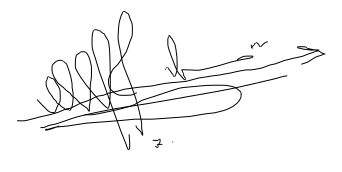
\includegraphics[width=0.8\linewidth]{\signature}\\ \\
	\textbf{Принял:} & \rang & \teacherfio 
\end{tabular}
\end{table}
\end{center}

\begin{flushleft}
	\begin{tabular}{p{0.25\linewidth}l}

		Работа выполена & <<\noindent\rule{2em}{1pt}>>
		                    \noindent\rule{5em}{1pt} 202\noindent\rule{1em}{1pt} \\

		<<Зачтено>> & <<\noindent\rule{2em}{1pt}>>
		\noindent\rule{5em}{1pt} 202\noindent\rule{1em}{1pt} \\

	\end{tabular}
\end{flushleft}

\normalsize
\begin{center}	
\vfill 
Москва 2021
\end{center}

	\newpage
	%\tableofcontents
	\newpage
	%\listoftables
\maketitle

\begin{table}[htbp]
\begin{center}
		\caption{Таблица адресации}
	\begin{tabular}{|l|l|l|l|}
		\hline
		Устройство  & Интерфейс & IP-адрес & Маска подсети \\ \hline
		S1 & VLAN 1 & 192.168.6.11 & 255.255.255.0 \\ \hline
		S2\_DENISOV & VLAN 1 & 192.168.6.12 & 255.255.255.0 \\ \hline
		PC-A & NIC & 192.168.6.3 & 255.255.255.0 \\ \hline
		PC-B & NIC & 192.168.6.2 & 255.255.255.0 \\ \hline
	\end{tabular}
	\label{tab:adress}
\end{center}
\end{table}

\mypart{Создание и настройка сети}
\step{Подключите все устройства в соответствии с топологией}
Построим топологию сети в соответствии с заданием (см. рис. \ref{fig:topology4}).
% TODO: \usepackage{graphicx} required
\begin{figure}[h!]
	\centering
	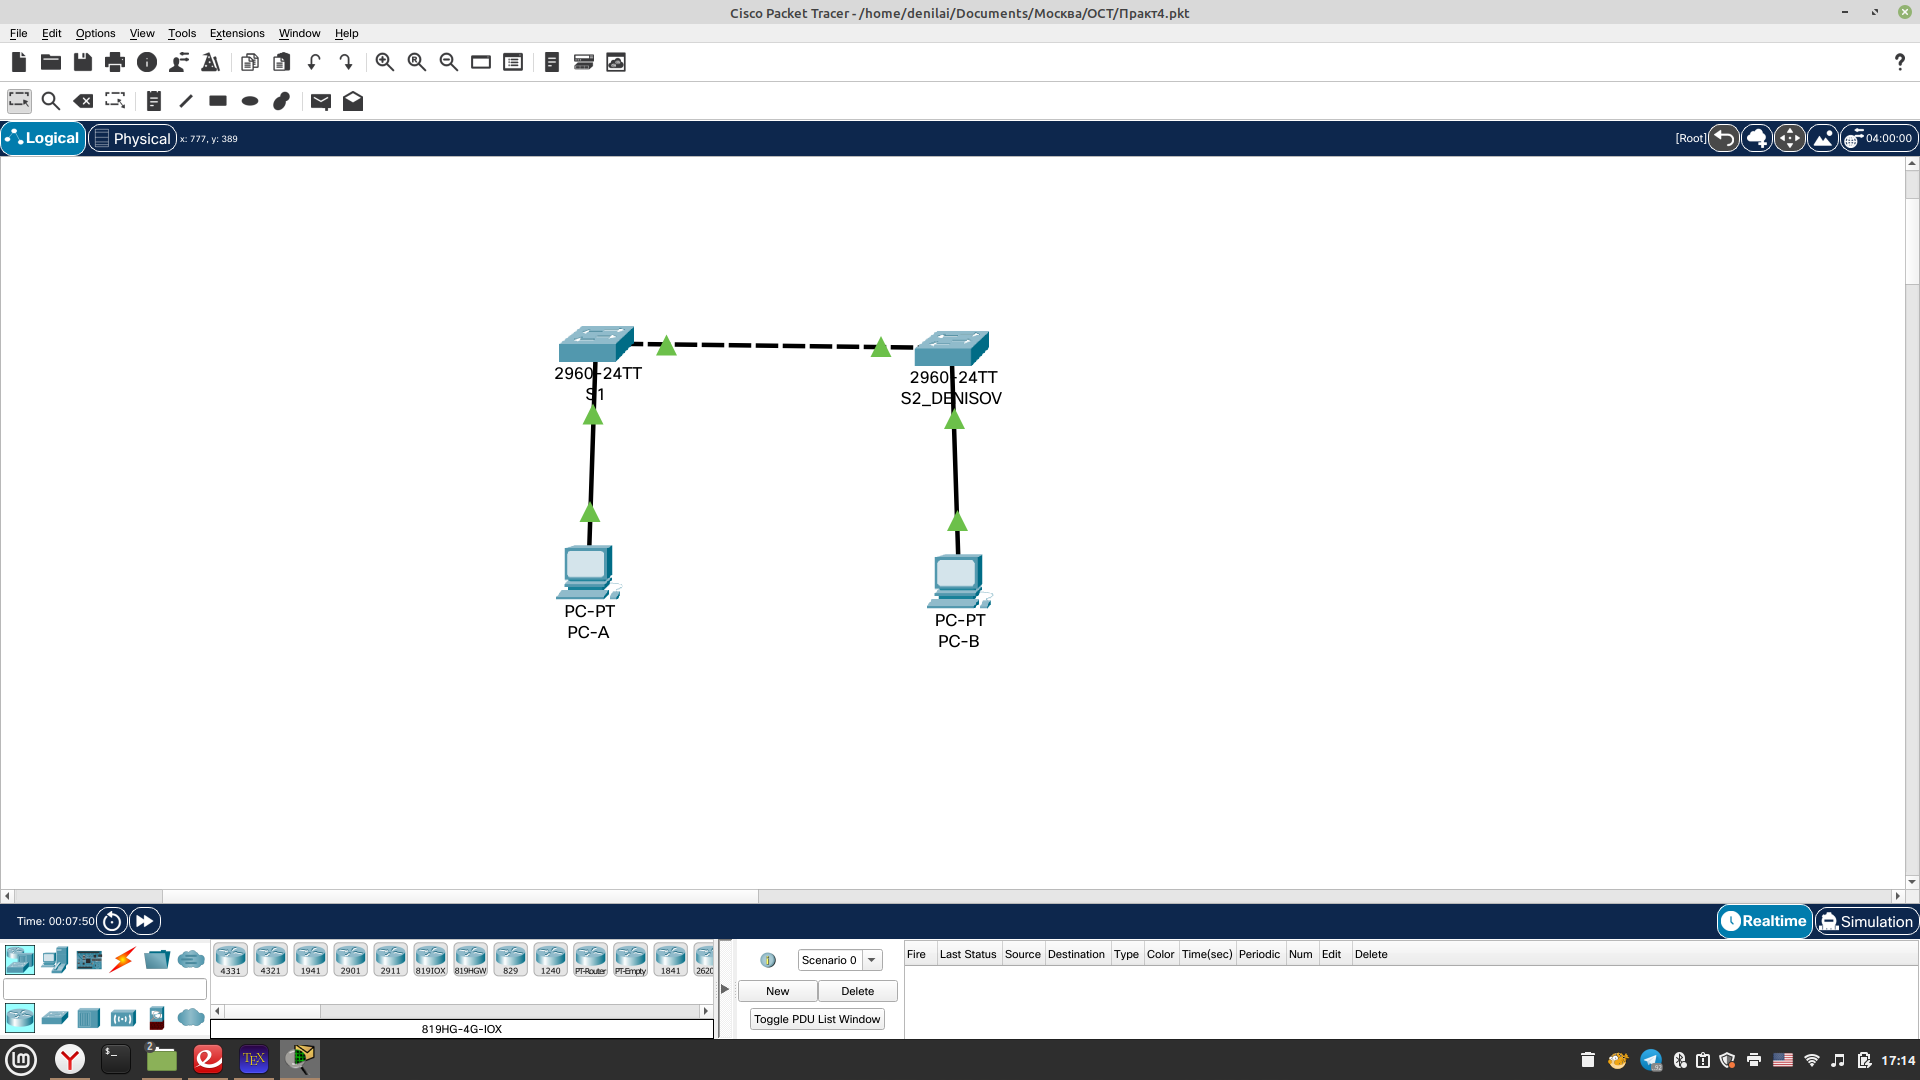
\includegraphics[width=0.7\linewidth]{images/topology4}
	\caption{Топология сети}
	\label{fig:topology4}
\end{figure}

\step{Настройте узлы ПК}
\step{Настройте базовые параметры каждого коммутатора}
\begin{enumerate}
	\item Настроим имена устройств в соответствии с топологией.
	\item Настроим IP-адреса, как указано в таблице адресации.
	\item Назначим cisco в качестве паролей консоли и VTY.
	\item Назначим class в качестве пароля привилегированного режима EXEC
\end{enumerate}
Приведем running configuration коммутаторов S1 и S2\_DENISOV, после проведения вышеописанных шагов.
Switch S1:
\begin{lstlisting}
	Building configuration...
	
	Current configuration : 1221 bytes
	!
	version 15.0
	no service timestamps log datetime msec
	no service timestamps debug datetime msec
	service password-encryption
	!
	hostname Switch
	!
	enable secret 5 $1$mERr$9cTjUIEqNGurQiFU.ZeCi1
	!
	!
	!
	!
	!
	!
	spanning-tree mode pvst
	spanning-tree extend system-id
	!
	interface FastEthernet0/1
	!
	interface FastEthernet0/2
	!
	interface FastEthernet0/3
	!
	interface FastEthernet0/4
	!
	interface FastEthernet0/5
	!
	interface FastEthernet0/6
	!
	interface FastEthernet0/7
	!
	interface FastEthernet0/8
	!
	interface FastEthernet0/9
	!
	interface FastEthernet0/10
	!
	interface FastEthernet0/11
	!
	interface FastEthernet0/12
	!
	interface FastEthernet0/13
	!
	interface FastEthernet0/14
	!
	interface FastEthernet0/15
	!
	interface FastEthernet0/16
	!
	interface FastEthernet0/17
	!
	interface FastEthernet0/18
	!
	interface FastEthernet0/19
	!
	interface FastEthernet0/20
	!
	interface FastEthernet0/21
	!
	interface FastEthernet0/22
	!
	interface FastEthernet0/23
	!
	interface FastEthernet0/24
	!
	interface GigabitEthernet0/1
	!
	interface GigabitEthernet0/2
	!
	interface Vlan1
	ip address 192.168.6.11 255.255.255.0
	!
	!
	!
	!
	line con 0
	password 7 0822455D0A16
	login
	!
	line vty 0 4
	password 7 0822455D0A16
	login
	transport input telnet
	line vty 5 15
	login
	!
	!
	!
	!
	end
	
	
	Switch#
\end{lstlisting}
Switch S2\_DENISOV:
\begin{lstlisting}
	Building configuration...
	
	Current configuration : 1241 bytes
	!
	version 15.0
	no service timestamps log datetime msec
	no service timestamps debug datetime msec
	service password-encryption
	!
	hostname Switch
	!
	enable secret 5 $1$mERr$9cTjUIEqNGurQiFU.ZeCi1
	!
	!
	!
	no ip domain-lookup
	!
	!
	!
	spanning-tree mode pvst
	spanning-tree extend system-id
	!
	interface FastEthernet0/1
	!
	interface FastEthernet0/2
	!
	interface FastEthernet0/3
	!
	interface FastEthernet0/4
	!
	interface FastEthernet0/5
	!
	interface FastEthernet0/6
	!
	interface FastEthernet0/7
	!
	interface FastEthernet0/8
	!
	interface FastEthernet0/9
	!
	interface FastEthernet0/10
	!
	interface FastEthernet0/11
	!
	interface FastEthernet0/12
	!
	interface FastEthernet0/13
	!
	interface FastEthernet0/14
	!
	interface FastEthernet0/15
	!
	interface FastEthernet0/16
	!
	interface FastEthernet0/17
	!
	interface FastEthernet0/18
	!
	interface FastEthernet0/19
	!
	interface FastEthernet0/20
	!
	interface FastEthernet0/21
	!
	interface FastEthernet0/22
	!
	interface FastEthernet0/23
	!
	interface FastEthernet0/24
	!
	interface GigabitEthernet0/1
	!
	interface GigabitEthernet0/2
	!
	interface Vlan1
	ip address 192.168.6.12 255.255.255.0
	!
	!
	!
	!
	line con 0
	password 7 0822455D0A16
	login
	!
	line vty 0 4
	password 7 0822455D0A16
	login
	transport input telnet
	line vty 5 15
	login
	!
	!
	!
	!
	end
\end{lstlisting}


\mypart{Изучение таблицы МАС-адресов коммутатора}
Как только между сетевыми устройствами начинается передача данных, коммутатор выясняет МАС-
адреса и строит таблицу.
\step{Запишите МАС-адреса сетевых устройств}
Откроем командную строку на PC-A и PC-B и введем команду \textit{ipconfig /all}. Приведем физические
адреса адаптера Ethernet. (см. рис. \ref{fig:mac-pac-a},\ref{fig:mac-pac-b}).
% TODO: \usepackage{graphicx} required
\begin{figure}[h!]
	\centering
	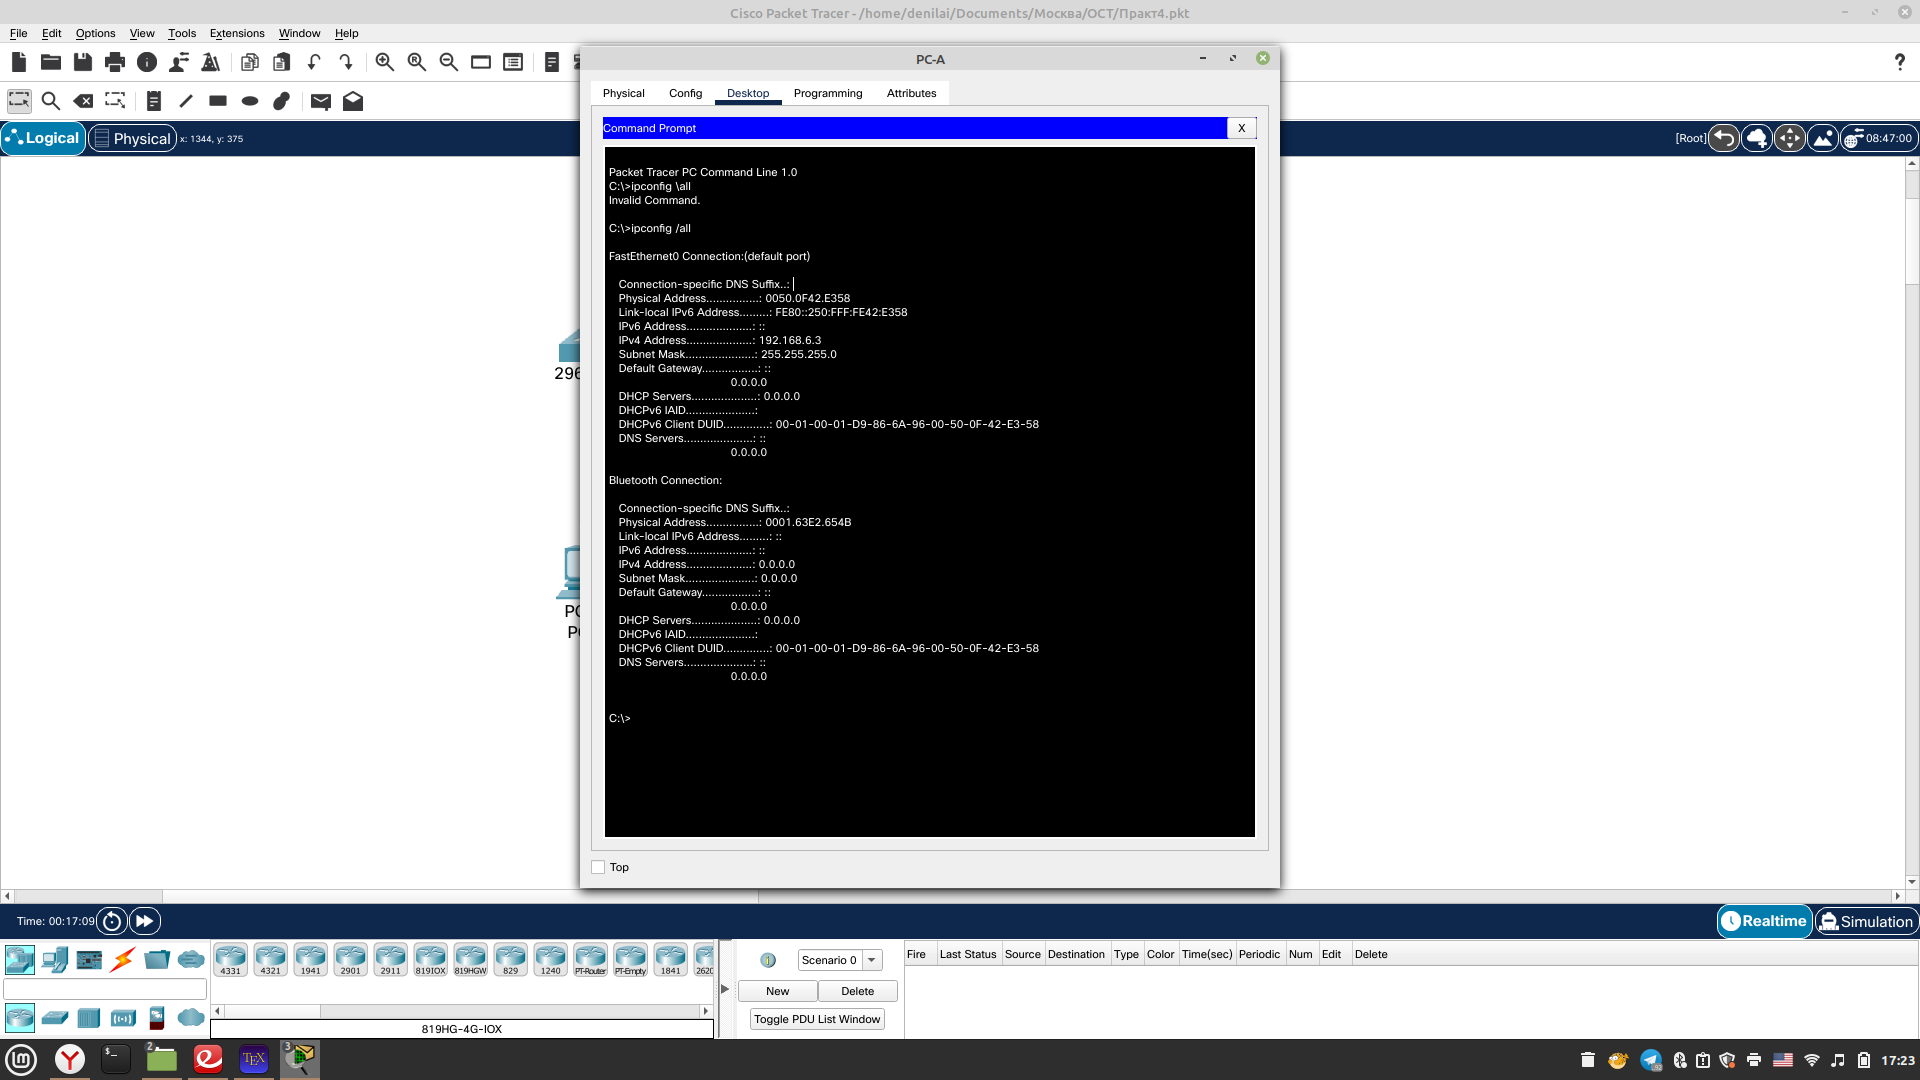
\includegraphics[width=0.7\linewidth]{images/mac-pac-a}
	\caption{Физический адрес компьютера PC-A}
	\label{fig:mac-pac-a}
\end{figure}
% TODO: \usepackage{graphicx} required
\begin{figure}[h!]
	\centering
	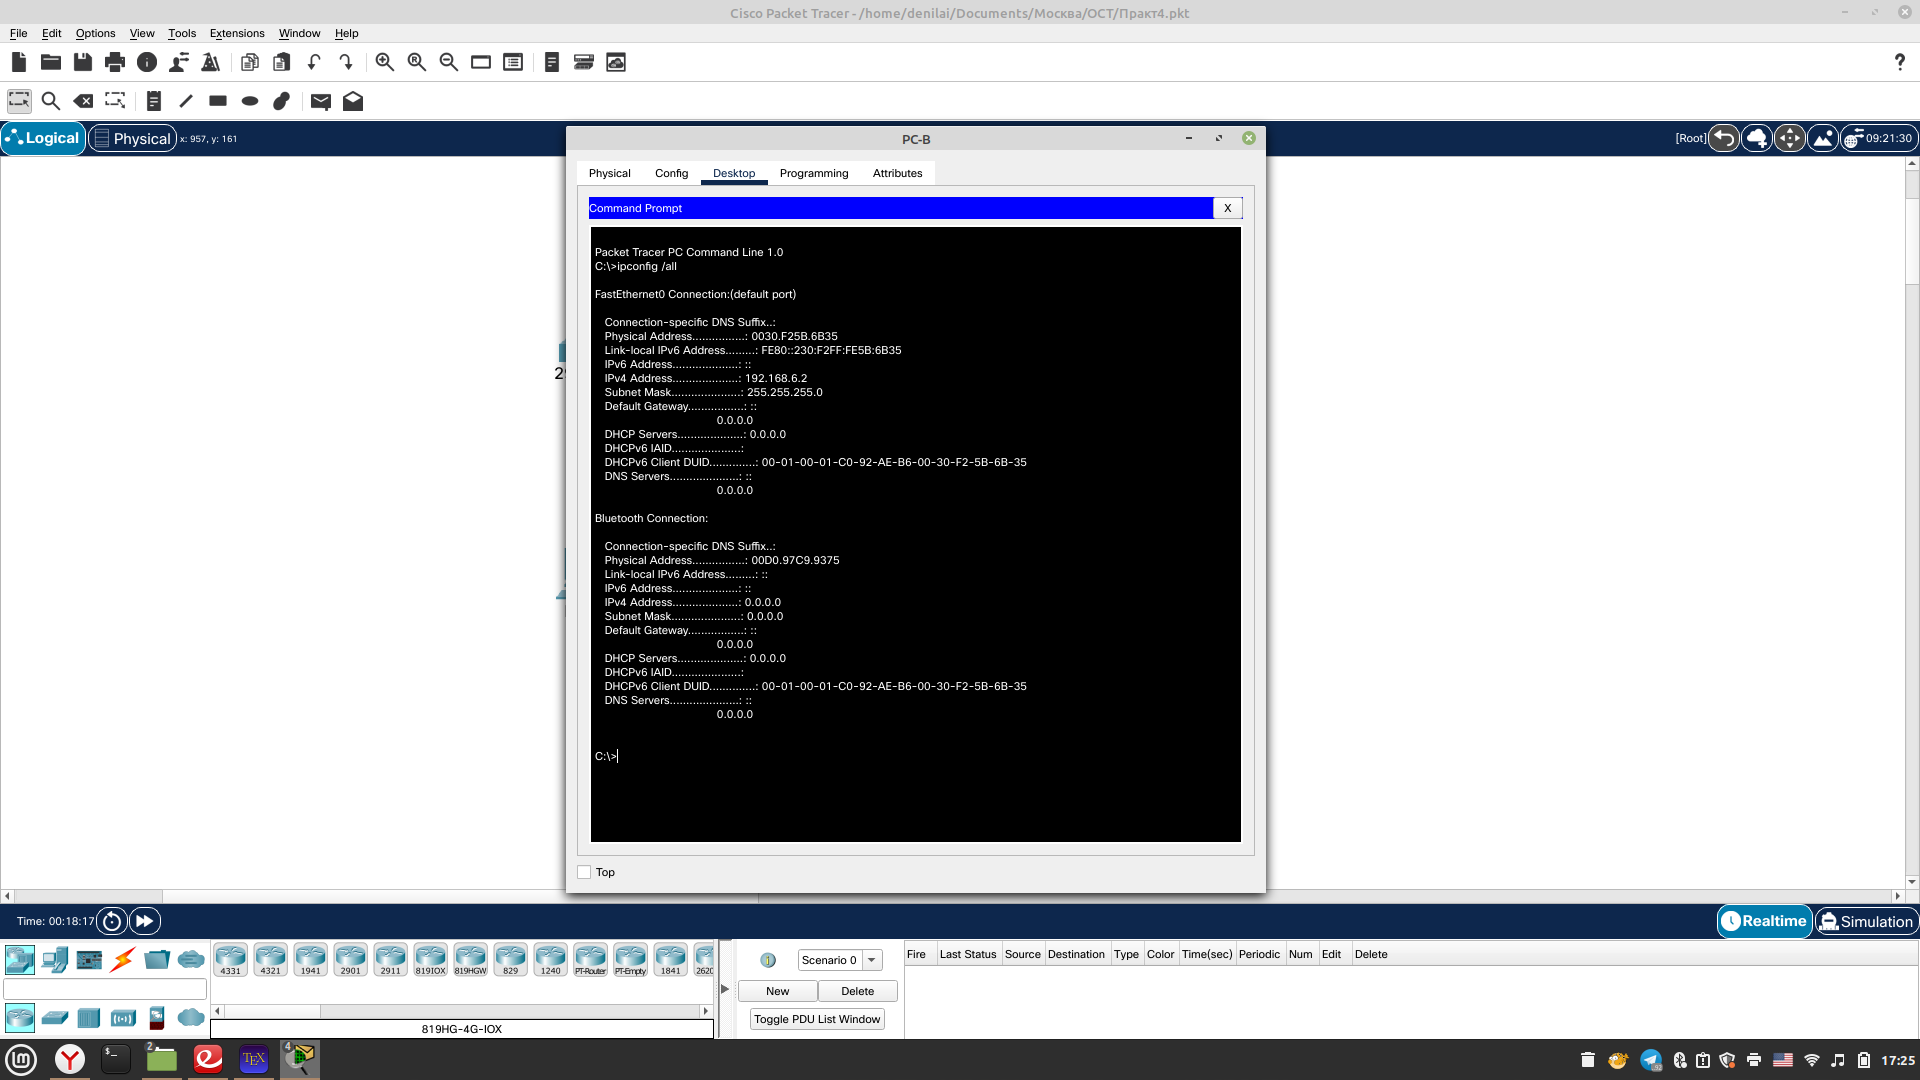
\includegraphics[width=0.7\linewidth]{images/mac-pac-b}
	\caption{Физический адрес компьютера PC-B}
	\label{fig:mac-pac-b}
\end{figure}

\begin{align*}
PC-A:& 0050.0F42.E358\\
PC-B:& 0030.F25B.6B35
\end{align*}

Какая часть MAC-адреса этого устройства соответствует OUI?

\begin{align*}
PC-A:& 0050.0F\\
PC-B:& 0030.F2
\end{align*}



Какая часть MAC-адреса этого устройства соответствует серийному номеру?

\begin{align*}
PC-A:& 42.E358\\
PC-B:& 5B.6B35
\end{align*}

Подключимся коммутаторам S1 и S2\_DENISOV через консоль и введем команду для
отображения MAC-адресов интерфейсов, задействованных в нашей топологии, на каждом
коммутаторе. 

Назовите адреса оборудования (или зашитый адрес — bia). Необходимо указать
адреса интерфейсов, с помощью которых соединяются 2 коммутатора
Коммутаторы соединяются с помощью интерфейсов FastEthernet 0/2
\begin{align*}
S1 &F0/2~bia: 0001.c798.5c02\\
S2\_DENISOV &F0/2~bia: 0090.2ba1.9702
\end{align*}

\step{Просмотрите таблицу МАС-адресов коммутатора}
Подключимся к коммутатору S2\_DENISOV через консоль и просмотрим таблицу МАС-адресов с помощью команды \textit{show mas-address-table} до и
после тестирования сетевой связи с помощью эхо-запросов. Ответим на вопросы:
\begin{enumerate}
	\item Записаны ли в таблице МАС-адресов какие-либо МАС-адреса? \\\textbf{Ответ} --- \textit{Да}
	\item Какие МАС-адреса записаны в таблице? С какими портами коммутатора они сопоставлены и каким
	устройствам принадлежат? Игнорируйте МАС-адреса, сопоставленные с центральным
	процессором.\\\textbf{Ответ} --- \textit{В таблице представлена одна запись. Она сопоставлена с портом F0/2 и принадлежит коммутатору S1}
	\item Если вы не записали МАС-адреса сетевых устройств в шаге 1, как можно определить, каким
	устройствам принадлежат МАС-адреса, используя только выходные данные команды для
	отображения таблицы MAC-адресов? Работает ли это решение в любой ситуации?\\
	\textbf{Ответ} --- \textit{сделать вывод о том, каким устройствам принадлежан MAC-адреса можно по столбцу "Ports" в выводе команды show mac-address-table. Этот способ работает, если мы имеем представление о строении логической топологии сети}
\end{enumerate}


\step{Очистите таблицу МАС-адресов коммутатора S2\_ФАМИЛИЯ и снова отобразите таблицу МАС-адресов}

В привилегированном режиме EXEC введем команду\textit{ clear mac address-table dynamic}.
\begin{lstlisting}
	S2# clear mac address-table dynamic
\end{lstlisting}

% TODO: \usepackage{graphicx} required
\begin{figure}[h!]
	\centering
	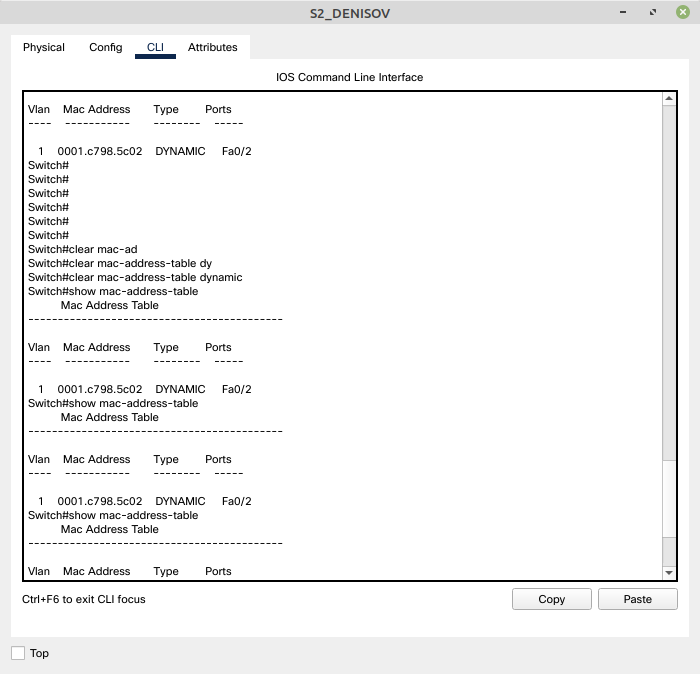
\includegraphics[width=0.6\linewidth]{images/clear-mac-s2}
	\caption{Очистка mac-address-table в S2\_DENISOV}
	\label{fig:clear-mac-s2}
\end{figure}
Снова быстро отобразим содержимой таблицы коммутации. 
Указаны ли в ней МАС-адрес для
VLAN 1? Указаны ли другие МАС-адреса?

\textbf{Ответ} --- \textit{нет, не указаны}

Через 10 секунд снова введите команду для отображения таблицы MAC-адресов и нажмите
клавишу ввода. Появились ли в ней новые адреса?

\textbf{Ответ} --- \textit{В таблице появились MAC-адреса, содержащиеся в ней до удаления}


\step{С компьютера PC-B отправьте эхо-запросы устройствам в сети и просмотрите
	таблицу МАС-адресов коммутатора}
\begin{enumerate}
	\item На компьютере PC-B откройте командную строку и введите команду для отображения ARP-кэша
	узла. Не считая адресов многоадресной и широковещательной рассылки, сколько пар IP- и МАС-адресов устройств было получено через протокол ARP?\\
	\textbf{Ответ} --- \textit{Две пары адресов. Для двух коммутаторов (см. рис. \ref{fig:arp-pc-b}).}
	% TODO: \usepackage{graphicx} required
	\begin{figure}[h!]
		\centering
		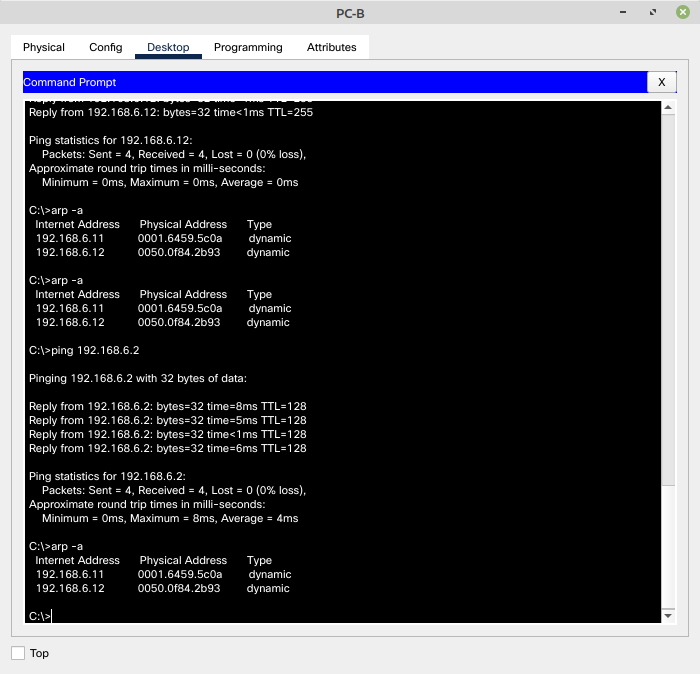
\includegraphics[width=0.5\linewidth]{images/arp-pc-b}
		\caption{Результат команды \textit{arp -a} на PC-B}
		\label{fig:arp-pc-b}
	\end{figure}
	
	\item Из командной строки PC-B отправьте эхо-запросы на компьютер PC-A, а также коммутаторы S1 и
	S2\_DENISOV. От всех ли устройств получены ответы?
	\\ \textbf{Ответ} --- \textit{Да, ответы получены от всех устройств в сети}
	\item Подключившись через консоль к коммутатору S2\_DENISOV, введите команду для отображения
	таблицы MAC-адресов. Добавил ли коммутатор в эту таблицу дополнительные МАС-адреса? Если
	да, то какие адреса и устройства?
	\\ \textbf{Ответ} --- \textit{Да, коммутатор добавил в таблицу два дополнительных MAC-адреса. Данные адреса принадлежат PC-A и PC-B (см. рис. \ref{fig:test-mac-b2}). }
	\item На компьютере PC-A откройте командную строку и еще раз введите команду из пункта «а».
	Появились ли в ARP-кэше компьютера PC-A дополнительные записи для всех сетевых устройств,
	которым были отправлены эхо-запросы?\\
	\textbf{Ответ} --- \textit{Да, появились сведения о всех остальных устройствах в сети (см. рис. \ref{fig:arp-pc-a}).}
		% TODO: \usepackage{graphicx} required
		\begin{figure}
			\centering
			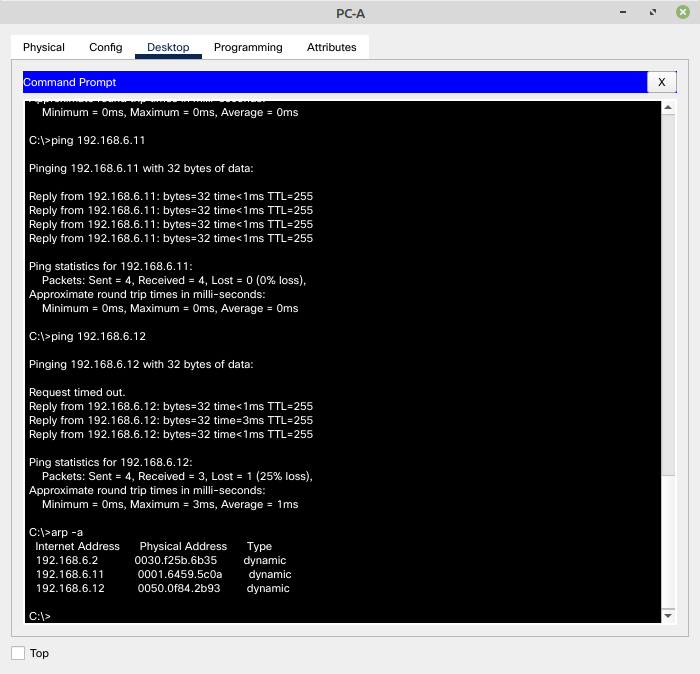
\includegraphics[width=0.5\linewidth]{images/arp-pc-a}
			\caption{Результат работы команды \textit{arp -a} на PC-A}
			\label{fig:arp-pc-a}
		\end{figure}
		
\end{enumerate}


% TODO: \usepackage{graphicx} required
\begin{figure}[h!]
	\centering
	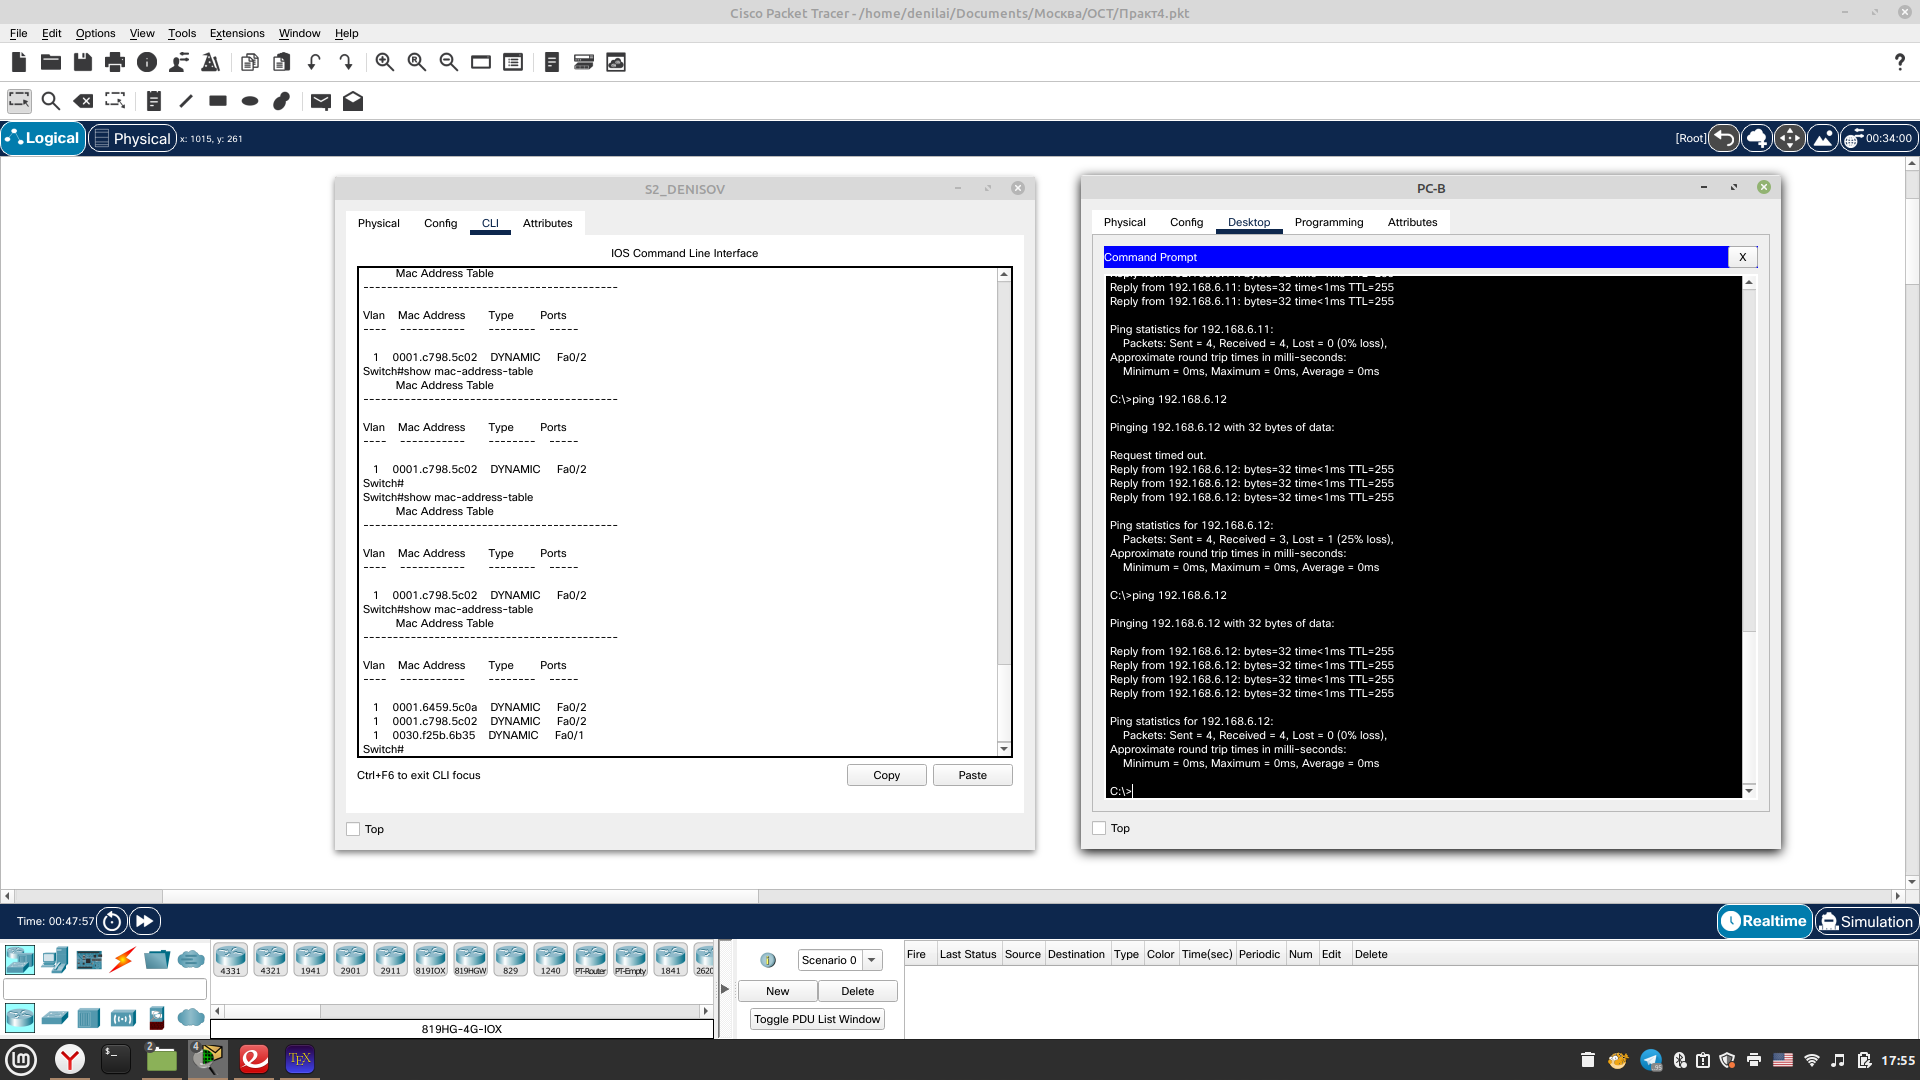
\includegraphics[width=0.8\linewidth]{images/test-mac-b2}
	\caption{}
	\label{fig:test-mac-b2}
\end{figure}



\mypart{Защита лабораторной работы (ответ на контрольные вопросы и вопросы
	преподавателя)}
\begin{enumerate}
	\item В сетях Ethernet данные передаются на устройства по соответствующим МАС-адресам. Для
	этого коммутаторы и компьютеры динамически создают ARP-кэш и таблицы МАС-адресов.
	Если компьютеров в сети немного, эта процедура выглядит достаточно простой. Какие
	сложности могут возникнуть в крупных сетях? 
	\\\textbf{Ответ} --- \textit{При большом количестве устройств в сети таблица MAC-адресов может переполнится, что приведет к выходу коммутатора из строя на некоторое время. Когда таблица МАС-адресов наполняется фиктивными МАС-адресами, коммутатор входит в так называемый режим с пропусканием трафика. В этом режиме коммутатор отправляет все кадры по широковещательной рассылке всем устройствам в сети. На данной уязвимости основана т.н. лавинная атака.}
	\item Можете ли вы использовать широковещательную рассылку на уровне 2? Если да, то каким
	будет ее MAC-адрес?
	\\ \textbf{Ответ} --- \textit{Да, можем. Адрес широковещательной рассылки на уровне 2 модели OSI --- FF-FF-FF-FF-FF-FF}
	\item Зачем нужно знать MAC-адрес устройства?
	\\ \textbf{Ответ} --- \textit{Если нужно организовать фильтрацию по MAC-адресам. Для получения информации о изготовителе прибора, номере его серии}
	\item Для чего нужен протокол ARP?
	\\ \textbf{Ответ} --- \textit{Протокол ARP позволяет автоматически определить МАК-адрес компьютера по его IP-адресу. Протокол работает в режиме запрос-ответ.}
\end{enumerate}




\end{document}



